\chapter{Method}


	
	
	% computer vision
	
	Points within a 3d point cloud are simply represented by their x, y, z Cartesian coordinates, with respect to a given origin. This means that there is a possibility that there are two points with the same x, y, z Cartesian coordinates that have been acquired at different times, this is assuming that the origin is the same. Comparing these points is not as easy as one would assume, they may occupy the same point in space, but who are we do assume that they are the same.
	
	We may get some extra data from a laser scanner, such as intensity and colour. But this doesn't really give us any more information about the area surrounding these points and weather anything has changed.
	
	Situations where points need to be compared for any reason require more information than can be provided by a laser scanner. So the idea of looking at each point individually now falls away. We need to start looking at the bigger picture of what the point cloud is telling us.
	

	

	
	
	\section{Region Growing}
	Point Cloud Libraries region growing algorithm starts off by calculating the curvature for each point then sorting all points by their curvature value. this is because the point with the least curvature associated with it is located in the flattest section of the point cloud. Once the cloud is sorted the region growing part of the algorithm begins:
	
	\renewcommand\labelitemi{{\boldmath$\cdot$}}
	\begin{itemize}
		\item The algorithm picks the point with the smallest curvature and adds it to a set called seeds.
		
		\item For every seed point the algorithm looks at all the neighbors and decides if they are part of that seeds region or not. This is done by looking at certain criteria with user specified thresholds.
		
		\begin{itemize}
			\item Does the points normal deviate by more than the user specified threshold from the seed point.
			
			\item Does the points curvature deviate by more than the user specified threshold from the seed point.
			
		\end{itemize}
		
		\item Once no more points are found for that particular seed, or the region reached a specified maximum, the seed is removed from the set of seeds and the region as added to the global segment list. If no more seeds are in the set the process is started from the beginning again, except this time the points that have been assigned to a region are no longer available to be seed points or to become part of a region.
		
	\end{itemize}
	
	If after a seed point has been through the process and the number of points does not reach the user defined minimum size the whole region removed from the cloud as unclassified and will inevitably be removed by the user.
	
	
	\begin{figure}[H]
		\centering
		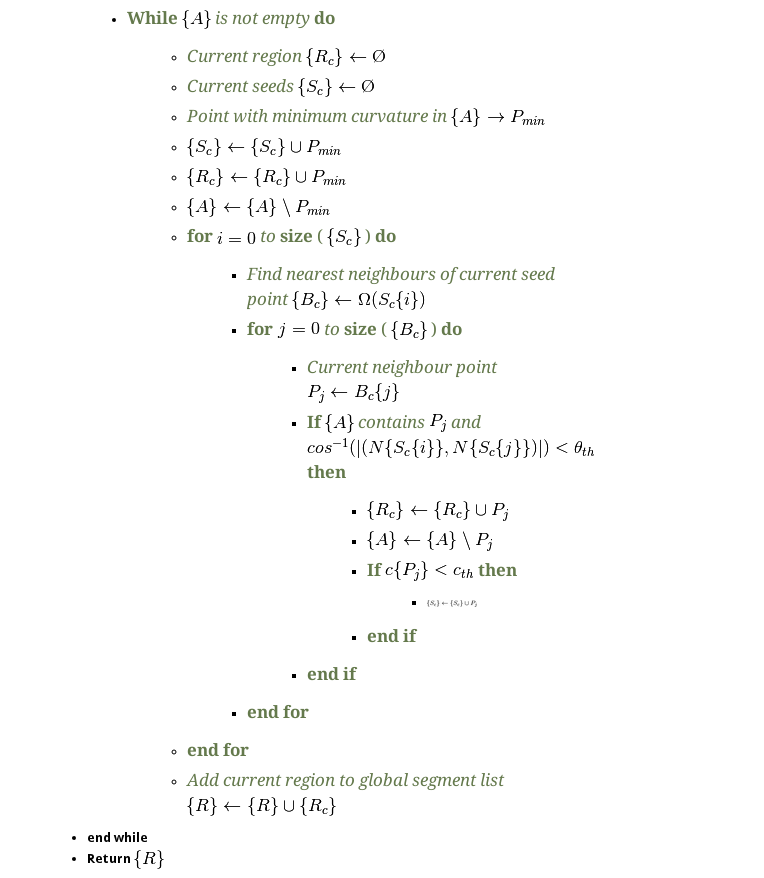
\includegraphics[width=0.7\linewidth]{Includes/images/LitReview/RegionGrowing}
		\caption{Pseudo code for region growing algorithm}
		\label{fig:RegionGrowing}
	\end{figure}
	
\section{Plane Fitting to Segments}

\section{Removal of Segments}

\section{Intersection of Planes}

\section{title}